\documentclass[xcolor=dvipsnames,hyperref={pdfpagelabels=false}]{beamer}

\usetheme{Boadilla}

\newcommand{\bi}{\begin{itemize}}
\newcommand{\ei}{\end{itemize}}
\newcommand{\be}{\begin{enumerate}}
\newcommand{\ee}{\end{enumerate}}
\newcommand{\bc}{\begin{center}}
\newcommand{\ec}{\end{center}}
\newcommand{\bd}{\begin{description}}
\newcommand{\ed}{\end{description}}
\newcommand{\I}{\item}
\newcommand{\f}{\frame}
\newcommand{\ft}{\frametitle}

\title{Offline Software Overview}
\subtitle{GlueX Collaboration Meeting}
\author[Mark Ito]{Mark M.\ Ito}
\date{June 5, 2013}
\institute[JLab]{Jefferson Lab}

\begin{document}

\f{\titlepage}

\f{\ft{Topics covered in other talks}
\bi
\I BCAL reconstruction, Will Levine, Calorimeter session
\I Tracking, Simon Taylor, Offline Software session
\I Translation tables, detector naming scheme, David Lawrence, Online session
\ei
}

\f{\ft{Progress 1}

\bi
\I Making REST skims (20-Mar)
  \bi
  \I Paul Mattione
  \I Allow users to optionally write REST-formatted data
  \I Useful for skims
  \ei
\I Simple Email Lists (20-Mar)
  \bi
  \I MMI
  \I Used for notification of nightly builds, b1pi test, single-track reconstruction test
  \I Limited audience
  \ei
\I Removal of hard-wired run numbers (20-Mar)
  \bi
  \I David Lawrence
  \I Rationalization
  \I Fixes consequence of pre-CCDB era: no run dependence for any constants
  \ei
\ei
}

\f{\ft{Progress 2}
\bi
\I HDDM changes (20-Mar)
  \bi
  \I Richard Jones
  \I Rationalization
  \I Explicitly separate known-only-by-simulation data from detector-based data
  \I Series of meeting to discuss changes
  \I Work in progress
  \ei
\I New version: JANA 0.6.6 (20-Mar)
  \bi
  \I David Lawrence
  \I support for resources, large, file-based data
  \I start-up time improvement for multi-threaded jobs
  \ei
\I Computer Resource Request (20-Mar)
  \bi
  \I David Lawrence, MMI
  \I Request from Graham Heyes, computing resources for FY14, 15, 16
  \I Used numbers from last year's Software Review
  \ei
\ei
}

\f{\ft{Computer Resource Request}
\begin{center}
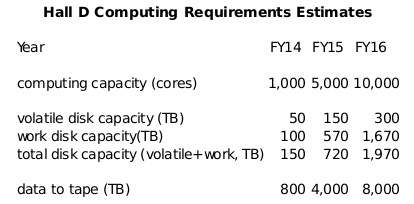
\includegraphics[width=0.8\textwidth]{computing_requirements_estimates.png} \\
{\bf Rough Cost Estimate} \\
\begin{tabular}{lr}
CPU & \$716 k \\
Disk & \$208 k \\
Tape & \$90 k \\
\hline
Total & \$1,014 k \\
\end{tabular}
\end{center}
}

\f{\ft{Progress 3}
\bi
\I Policy on Virtual machines at JLab (20-Mar)
  \bi
  \I Andy Kowalski (JLab IT Division)
  \I Draft only so far
  \I VMWare platform provided by IT Division
  \I Only approved OS images can be installed on user machines
  \ei
\I RF bunch selection (3-Apr)
  \bi
  \I Paul Mattione
  \I Prototype system available
  \I Specify event topology first
  \I Only particles that fit topology used in bunch selection
  \ei
\I Another Alternate BCAL Reconstruction Algorithm (3-Apr)
  \bi
  \I Beni Zihlmann
  \I Tool to understand issues
  \I Will be made publicly available
  \ei
\ei
}

\f{\ft{Progress 4}
\bi
\I Standard ROOT TTree Format (17-Apr)
  \bi
  \I Paul Mattione
  \I For reconstructed results
  \I Easy ROOT-friendly access to quantities
  \I Multiple particle combinations for a given topology supported
  \I Intended for general physics analysis
  \ei
\I Smearing beam particle momentum in genr8\_2\_hddm (17-Apr)
  \bi
  \I David Lawrence
  \I Optional
  \ei
\I Rationalization of particle numbers in HDGeant (17-Apr)
  \bi
  \I David Lawrence
  \I Make consistent with GEANT documentation
  \ei
\ei
}

\f{\ft{Things to Do This Summer}
\bi
\I Geant4 conversion (1-May)
  \bi
  \I Richard Jones
  \ei
\I The Next Data Challenge (1-May)
  \bi
  \I Many issues left over from last one (see next slide)
  \ei
\I Code profiling regimen
  \bi
  \I Recommended by Software Review Committee
  \ei
\I Offline Task List/Project Management
  \bi
  \I Some tasks already done, need to systematize addressing un-done tasks
  \ei
\ei
}

\f{\ft{Next Data Challenge}
\bi
\I New software
  \bi
  \I fix bugs: improve job success efficiency 
  \I BCAL reconstruction
  \I CCDB
  \I latest tracking
  \I ROOT trees?
  \I improved REST?
  \ei
\I Simulation Configuration Changes
  \bi
  \I add electromagnetic background
  \I add in dark noise in the BCAL
  \I open up photon window, especially to higher photon energy, perhaps 7.5 GeV to the end-point
  \ei
\I System Improvements
  \bi
  \I farm management system at JLab
    \bi
    \I crude set of perl scripts now, full of kludges
    \I needs generalization, perhaps re-write
    \ei
  \I input and output data cataloging and management
    \bi
    \I database application?
    \I grid-based meta-data catalog?
    \ei
  \ei
\ei
}

\f{\ft{Upcoming Events}

\bi
\I Software Workshop -- July 10-11, 2013 (Wed., Thu.)
\I 12 GeV Software Review II -- September 2013
\ei
}

\end{document}
%%%%%%%%%%%%%%%%%%%%%%%%%%%%%%%%%%%%%%%%%%%%%%%%%%%%%%%%%%%%%%%%
